%%%%%%%%%%%%%%%%%%%%%%%%%%%%%%%%%%%%%%%%
%% HiMCM/MidMCM LaTeX Template -- 2026 %%
%% CP-SET Framework -- complete five-task manuscript
%% Efficiency/effectiveness scope separation, November 8, 2026.
%%%%%%%%%%%%%%%%%%%%%%%%%%%%%%%%%%%%%%%%
\documentclass[12pt]{article}
\usepackage{geometry}
\geometry{left=1in,right=0.75in,top=1in,bottom=1in}
\newcommand{\Problem}{B}
\newcommand{\Team}{18588}
\usepackage{newtxtext}
\usepackage{amsmath,amssymb,amsthm}
\usepackage{newtxmath}
\usepackage[pdftex]{graphicx}
\usepackage{xcolor}
\usepackage{fancyhdr}
\usepackage{microtype}
\usepackage{xurl}
\usepackage{needspace}
\usepackage{booktabs,tabularx,array}
\usepackage{enumitem,titlesec,caption,multicol,tocloft,float,placeins}
\usepackage[hidelinks]{hyperref}
\newif\ifinlineai
\inlineaitrue
\captionsetup{font=small,labelfont=bf,skip=4pt}
\titlespacing*{\section}{0pt}{10pt plus2pt minus1pt}{5pt}
\titlespacing*{\subsection}{0pt}{8pt plus1pt minus1pt}{3pt}
\setlength{\textfloatsep}{9pt plus2pt minus2pt}
\setlength{\floatsep}{7pt plus1pt minus1pt}
\setlength{\intextsep}{8pt plus1pt minus1pt}
\setcounter{topnumber}{5}
\setcounter{bottomnumber}{4}
\setcounter{totalnumber}{8}
\renewcommand{\topfraction}{.95}
\renewcommand{\bottomfraction}{.9}
\renewcommand{\textfraction}{.05}
\renewcommand{\floatpagefraction}{.85}
\setlength{\headheight}{15pt}
\setlength{\parskip}{1.5pt}
\setlength{\parindent}{1.2em}
\widowpenalty=10000
\clubpenalty=10000
\lhead{Team \Team}
\rhead{}
\cfoot{}
\newtheorem{theorem}{Theorem}
\newtheorem{corollary}[theorem]{Corollary}
\newtheorem{lemma}[theorem]{Lemma}
\newtheorem{definition}{Definition}

\begin{document}
\graphicspath{{.}}
\DeclareGraphicsExtensions{.pdf,.jpg,.png}
\thispagestyle{empty}
\vspace*{-16ex}
\centerline{\begin{tabular}{*3{c}}
\parbox[t]{0.3\linewidth}{\begin{center}\textbf{Problem Chosen}\\ \Large \Problem\end{center}}&
\parbox[t]{0.3\linewidth}{\begin{center}\textbf{2026\\ HiMCM/MidMCM\\ Summary Sheet}\end{center}}&
\parbox[t]{0.3\linewidth}{\begin{center}\textbf{Team Control Number}\\ \Large \Team\end{center}}\\
\hline
\end{tabular}}

\begin{center}
\vspace{1.1em}
{\Large\bfseries CP-SET: Measuring Useful Cooling\\in Open Public Spaces}\\[.5em]
{\bfseries Summary}
\end{center}
An open cooling system should be judged by the useful service reaching its users. We develop the \textbf{Coupled Psychrometric-SET Service Efficiency \& Effectiveness Framework (CP-SET)} to connect heat and moisture balances, local air delivery, human thermal response and operational decisions.

The freezer case establishes four essential quantities: service quantity, local quality, duration and electrical input. Its useful storage service motivates a human-service analogue: signed SET-excess relief accumulated over passenger-hours, divided by the electricity used by every operating device. This distinguishes efficiency from the adequacy of the cooling delivered.

For a New York City bus-shelter geometry, the framework combines wet-bulb-limited evaporation, dry-air-weighted local mixing and Standard Effective Temperature. At $34^\circ$C, fan A achieves efficiencies of $84.58$ and $90.57$ person$\cdot{}^\circ$C$\cdot$h/kWh at $30\%$ and $70\%$ RH. B and C require $4.8$ and $10$ times A's accumulated relief to overcome their power ratios. A delivery-loss test identifies where B overtakes A. A separate hot-dry test shows why larger thermal improvement need not imply higher efficiency.

At Canberra MRT station, the same delivery and response modules are retained while zone enthalpy, humidity and surface temperature evolve with exchange, passenger loads and equipment operation. Across 24 sampled installations, A3 reaches the highest efficiency, $37.58$; among six equal-coverage benchmarks, A36 leads at $35.49$. Relocating the same AB30 inventory toward passenger demand raises its efficiency from $15.39$ to $18.39$. Coverage and local delivery therefore matter alongside the rated cooling effect.

At \textbf{Fremont Street Experience} and the \textbf{Honolulu Zoo ticket queue}, modeled service areas differ by a factor of $139.7$. Largest-fitting pure A/B/C plans achieve efficiencies of $11.88/5.06/5.72$ and $47.71/21.28/20.63$, respectively. A controlled climate exchange confirms the B--C reversal. An energy-weighted bound establishes each site's maximum efficiency, while scale and boundary tests separate device replication from lost coverage and clipped delivery.

Extending the same physical outputs to thermal performance, visitor access, annual energy and cost gives an integer allocation problem. The stated operator policy selects A266C16 in Fremont and A1B1 in Honolulu, at equivalent annual costs of USD $50{,}926$ and $627$. In Honolulu, relaxing required mean relief from $1.50$ to $1.49^\circ$C selects three fans instead: the cost-minimizing choice depends on the service threshold.

Conservation checks, limiting-case recovery and time-step refinement verify the numerical implementation. Climate, local delivery and cost sensitivities identify the assumptions that affect the decision. The resulting memorandum and public explanation translate useful cooling per kWh into equipment placement, operating schedules and extreme-heat procedures.

\noindent\textbf{Keywords:} psychrometrics; local air delivery; Standard Effective Temperature; cooling service efficiency; multi-objective decisions.

\newpage
\pagestyle{fancy}\rhead{Page \thepage}
\setcounter{tocdepth}{1}
\section*{Contents}
{\fontsize{10}{11.5}\selectfont
\setlength{\cftbeforesecskip}{1pt}
\begin{multicols}{2}
\makeatletter\@starttoc{toc}\makeatother
\end{multicols}}
\vspace{4pt}
\section{Introduction}
\label{sec:introduction}
\subsection{Background}
Open cooling systems must deliver relief despite continuous exchange with their surroundings. Fans alter human convective and evaporative losses; evaporative coolers also change air temperature and moisture \cite{fanguide,evapequip}. Comparing them requires useful service per unit energy.

\subsection{Problem Restatement}
The five tasks are to define cooling efficiency, develop bus and rail models, test two contrasting venues, extend efficiency into an effectiveness decision, and communicate operating guidance through a memorandum and public blog \cite{problem}.

\subsection{Our Modeling Framework}
Our \textbf{CP-SET Framework (Coupled Psychrometric-SET Service Efficiency \& Effectiveness Framework)} connects conserved heat and moisture to local exposure, then converts SET relief into person-time service per kWh. Requirements 1--3 compare efficiency; Requirement 4 adds cooling adequacy, visitor experience and cost. The workflow below preserves this progression.
\begin{center}
\includegraphics[width=\linewidth]{figures/29_cp_set_framework.pdf}\\[-2pt]
{\small\textbf{CP-SET workflow.} A shared physical and service model supports progressively broader decisions.}
\end{center}
\ifinlineai
\noindent\footnotesize AI assistance in model development, coding and writing is documented in the appended report \cite{codex,gemini}.\normalsize
\fi
\clearpage
\section{Assumptions and Justifications}
\begingroup\setlength{\intextsep}{4pt}
\label{sec:assumptions}
\begin{enumerate}[leftmargin=*,itemsep=2pt,topsep=2pt,label=\textbf{A\arabic*.}]
\item \textbf{Matched service boundary.} Comparisons share weather, people, geometry and period; the problem's kW/hr entries are interpreted as kW. \textit{Justification:} A common workload and complete device-energy accounting isolate strategy efficiency.
\item \textbf{Zoned air and rapid local mixing.} Zones have uniform background states; local supply mixes at negligible storage, with disjoint footprints and separately prescribed speed. \textit{Justification:} This resolves occupied-location differences when local residence time is short relative to the 120-s station disturbance.
\item \textbf{Conserved heat and water.} Evaporation is near-adiabatic; background dry-air mass is fixed and exchange is balanced; shaded radiation uses mean radiant temperature. Condensation is excluded in public-space cases. \textit{Justification:} These approximations retain the dominant transfers while counting every electrical and vapor-enthalpy source once.
\item \textbf{Reference human response.} SET uses standing transport users and venue visitors at 1.2 met and 0.5 clo, with a $26^\circ$C excess reference. \textit{Justification:} One signed-relief measure compares airflow and evaporation. Dry-heat tests use $T_a=T_r=39/40^\circ$C and RH $15/20\%$: $40^\circ$C is the implementation boundary; the interior $39^\circ$C test retains the ranking \cite{pythermal}.
\item \textbf{Explicit design inputs.} Published sources establish site geometry and climate context; tabulated estimates specify operating and economic conditions. \textit{Justification:} Reproducible inputs support sensitivity analysis. Costs use one currency and horizon; equipment clearance is the visitor-access proxy. SET relief and operational heat-safety procedures serve separate purposes.
\end{enumerate}


\begin{table}[H]
\centering\fontsize{9.5}{10.7}\selectfont
\caption{Transport-case inputs. Geometry sources are cited; remaining entries are model design assumptions.}
\label{tab:bus-assumptions}\label{tab:rail-inputs}
\begin{tabularx}{\linewidth}{@{}p{.18\linewidth}XX@{}}
\toprule
Input & Bus shelter & Canberra waiting area\\
\midrule
Geometry & $4.2672\times1.5240\times2.7178$ m \cite{nycshelter}; three equal gross strips & $L=220$ m \cite{canberra-dimensions}; effective waiting width $6$ m, usable fraction $.8$, air height $4$ m; three zones\\
Climate / radiation & $T_a=34^\circ$C; RH $30/70\%$; $T_r=36^\circ$C & $T_o=33^\circ$C, RH $70\%$; external $T_{r,o}=33^\circ$C \cite{singapore-climate}\\
People / time & $(4,4,4)$ people, 1 h; redistribution $(8,3,1)$ or $(1,3,8)$ & $(26.4,44,17.6)\to(88,198,66)$ linearly per 15-min cycle; 2-h warm-up + 2-h evaluation\\
Exchange & Fixed outdoor background & ACH $(8,4,10)$ plus $(8,4,12)$ in last 2 min; adjacent flow $.88$ kg dry air/s\\
Surface / people & Prescribed radiant conditions & Per zone $C_m=17.6$ MJ/K; $H_{ma}/H_{mo}=880/1760$ W/K; absorbed load $3520$ W; $F=(.55,.85,.55)$; per person $q_c/q_r=45/30$ W, $g=45/(2.45\times10^6)$ kg/s\\
Device delivery & Profiles in Table~\ref{tab:bus-fields}; $\chi=0$; $\chi$ sensitivity uses A $\beta=(.8,.45,.1)$ and rail flows & $\beta=.5$, $\chi=1$; A/B/C flow $.6/.6/1.2$ kg dry air/s; footprints $20/30/40$ m$^2$\\
Shared response & \multicolumn{2}{p{.77\linewidth}@{}}{Pressure $101325$ Pa; $v_0=.2$ m/s; body area $1.8258$ m$^2$, external work zero; $\varepsilon_{B/C}=.7$; outlet drops capped at $5/8^\circ$C. $\Theta_c$ sensitivity $24/26/28^\circ$C.}\\
\bottomrule
\end{tabularx}
\end{table}
\begin{table}[H]
\centering\fontsize{9.5}{10.7}\selectfont
\caption{Local speed and mixing profiles in zone order; each entry describes an independent local state.}
\label{tab:bus-fields}
\begin{tabular}{@{}lccc@{}}
\toprule
Device & Bus speed (m/s) & Bus $\beta_{s,z}$ & Rail covered speed (m/s)\\
\midrule
A & $1/.55/.25$ & Immaterial at $\chi=0$ & $.60/1/.50$\\
B & $.80/.50/.30$ & $.80/.45/.10$ & $.50/.80/.45$\\
C & $1/.80/.50$ & $.90/.70/.40$ & $.75/1/.60$\\
\bottomrule
\end{tabular}
\end{table}

\endgroup
\clearpage
\IfFileExists{sections/venue_assumptions.tex}{\begin{table}[H]
\centering\fontsize{9.5}{10.7}\selectfont
\caption{Venue design inputs. The canopy length and site identities are sourced; occupied width, queue area, weather snapshots, attendance, delivery and prices are planning assumptions.}
\label{tab:venue-inputs}
\begin{tabularx}{\linewidth}{@{}p{.18\linewidth}XX@{}}
\toprule
Input & Fremont Street Experience & Honolulu Zoo ticketing queue\\
\midrule
Service boundary & $419.1$-m canopy \cite{fremont-canopy}; assumed $20$-m occupied width; $A_z=(2400,3600,2382)$ m$^2$ & Window-side shaded public queue \cite{honolulu-zoo-entrance,honolulu-zoo-admission}; one assumed $10\times6$ m demand area\\
Climate / radiation & $T_a/T_r=38/39^\circ$C; RH $20\%$; $v_0=.20$ m/s \cite{las-vegas-climate} & Warm, weak-wind case: $31/33^\circ$C; RH $65\%$; $v_0=.35$ m/s \cite{honolulu-climate}\\
Hourly occupancy & $(120,240,90)$; $(180,480,150)$; $(240,720,180)$; $(180,480,150)$ & $12,24,36,24$ simultaneous visitors over four successive one-hour intervals\\
Common physics & \multicolumn{2}{p{.79\linewidth}@{}}{Prescribed outdoor background; $\chi=0$; standing visitors, 1.2 met, .5 clo. Each complete device footprint has three equal-area delivery strips with Table~\ref{tab:bus-fields}'s bus $\beta$ values and $v=v_0+(v_{\rm bus}-.20)$ m/s. Uniform density within each demand zone; disjoint footprints.}\\
Unit A/B/C & \multicolumn{2}{p{.79\linewidth}@{}}{Footprints $20/30/40$ m$^2$; flow $1.2/2/3$ kg$_{da}$/s; clearance $.5/1/1.5$ m$^2$; capital USD $300/1000/2000$; annual maintenance USD $30/100/200$.}\\
Operating basis & \multicolumn{2}{p{.79\linewidth}@{}}{$H=4$ h/session; $H_y=600$ h/y; equipment life 5 y, discount 5\%, zero salvage; USD $.20$/kWh and $3$/m$^3$; make-up-water factor $1.15$.}\\
Task 4 policy & \multicolumn{2}{p{.79\linewidth}@{}}{$q\ge.80$; mean SET-excess relief $\ge1.5^\circ$C; clearance fraction $X\le.035$; annual energy $\le30\sum_z A_z$ kWh. These conditions enter only the effectiveness decision.}\\
Transfer tests & \multicolumn{2}{p{.79\linewidth}@{}}{Exchange the complete weather tuple at fixed geometry/attendance; scale area and attendance together; clip a single device's far-to-near strips only in the separate boundary test. RH, radiant temperature, natural speed and area are varied individually.}\\
\bottomrule
\end{tabularx}
\end{table}
}{}
\input{sections/nomenclature}
\clearpage
% Requirements 1 and 2(a); numbered equations retain their original order.
\section[Freezer: service efficiency]{Understanding Cooling Efficiency}
\label{sec:understand}

An open freezer succeeds by preserving food, not simply by removing heat. Low electricity use can accompany inadequate storage, while large cooling loads may reflect infiltration through the opening. We therefore evaluate \emph{useful service per unit energy}.

\begin{figure}[!ht]
\centering
\begin{minipage}[c]{0.48\linewidth}
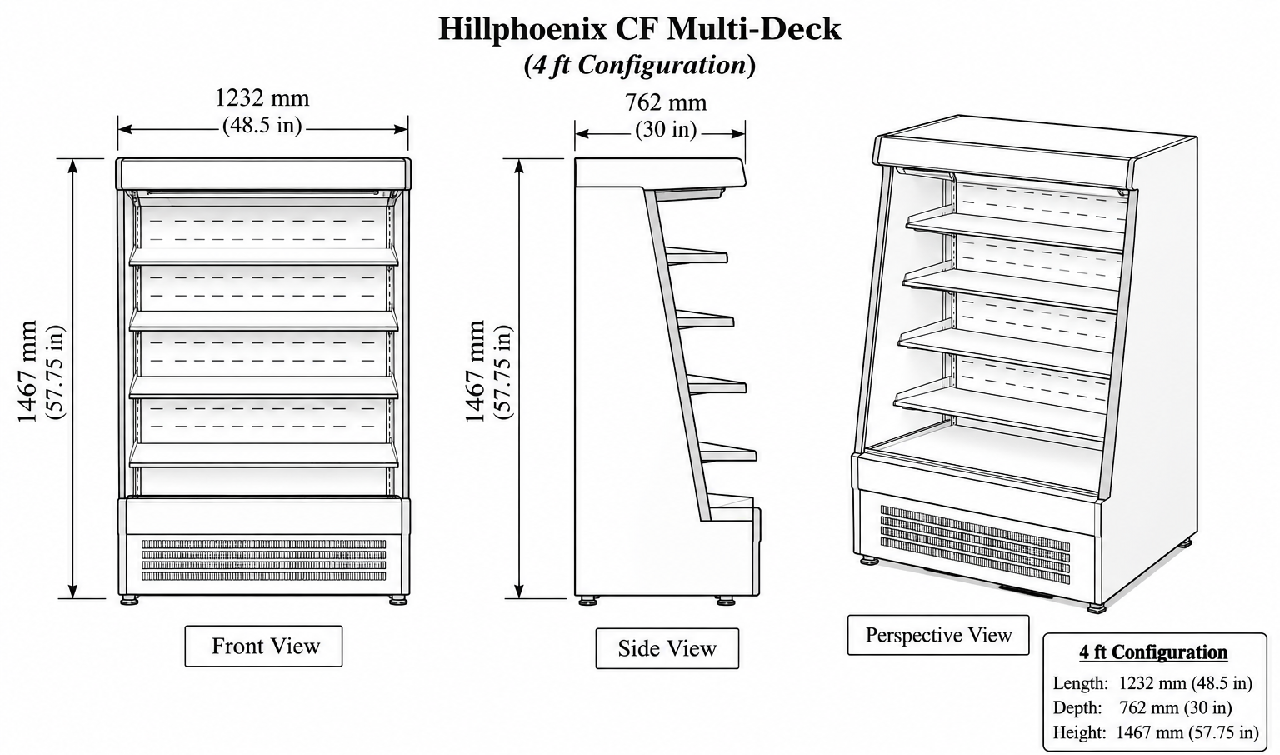
\includegraphics[width=\linewidth]{figures/09_open_display_case.pdf}
\end{minipage}\hfill
\begin{minipage}[c]{0.48\linewidth}
\small
The open front admits warm, moist air; cabinet surfaces conduct and radiate heat. Lights, fans, restocking and defrost add operating loads. Insulation and equipment condition modify these mechanisms; equipment age is not a separate score \cite{ashrae}. Product temperatures must be checked across shelves, since a mean can conceal a warm location \cite{etl}.
\end{minipage}
\caption{Open-case heat pathways and product locations. The supplied medium-temperature display schematic illustrates geometry; freezer limits remain product-specific \cite{hillphoenix}.}
\label{fig:open-case}
\end{figure}

The numerator needs \textbf{quantity, local quality and duration}: compliant product mass integrated over storage time. The denominator includes refrigeration and auxiliaries without overlapping meter readings. Matched loading, ambient conditions and complete operating cycles prevent short operation or stored cold from inflating efficiency:
\begin{equation}
\boxed{\text{Cooling efficiency}
=\frac{\text{useful service accumulated over objects and time}}
{\text{energy input over the same period}}.}
\label{eq:principle}
\end{equation}
\begin{equation}
 \eta_f=\frac{\int\sum_i m_i(t)\mathbf{1}\{T_{p,i}(t)\in\mathcal T_i\}\,dt}
 {\int p_f(t)\,dt},
\label{eq:freezer-service}
\end{equation}
Here $m_i$ is product mass (kg), $\mathcal T_i$ its admissible temperature range, $t$ is hours and $p_f$ is kW; thus $\eta_f$ is compliant kg$\cdot$h/kWh. For people, the response changes to thermal-discomfort relief weighted by occupied time. These recipient-specific numerators cannot be directly compared numerically.

\subsection{A shared physical structure}
For dry-air mass $M_z$ (kg), balanced dry-air streams $\dot m_{jz}$ (kg/s), enthalpy $h$ (J/kg dry air) and humidity ratio $w$ (kg vapor/kg dry air),
\begin{align}
 M_z\dot h_z&=\sum_j\dot m_{jz}(h_j-h_z)+S_{h,z},\\
 M_z\dot w_z&=\sum_j\dot m_{jz}(w_j-w_z)+S_{w,z}.
\label{eq:common-balance}
\end{align}
$S_h$ (W) and $S_w$ (kg/s) contain the appropriate device, occupant, product and surface sources. Freezer refrigeration can remove heat and condensate; public cooling changes airflow and moisture. The bus fixes the background and solves local delivery; the station retains that calculation while resolving background and surface storage \cite{epzone}. Figure~\ref{fig:inheritance} shows this progression. Cruz-Salas et al.\ motivate separating treatment, transport and occupied-space conditions \cite{cruz2026}.

\begin{figure}[!ht]
\centering
\includegraphics[width=0.94\linewidth]{figures/19_model_inheritance.pdf}
\caption{Shared conservation and service accounting, with recipient-specific response and increasingly resolved background dynamics.}
\label{fig:inheritance}
\end{figure}

\section[Bus shelter]{Bus Stop: Local Delivery and Cooling Efficiency}
\label{sec:bus}

\subsection{Geometry and comparison inputs}
NYC DOT's regular shelter measures $14$ ft by $5$ ft by $8$ ft $11$ in, or $4.2672\times1.5240\times2.7178$ m \cite{nycshelter}. Its gross footprint is $A=6.5032\,\mathrm{m^2}$. Three equal strips have $A_z=2.1677\,\mathrm{m^2}$ and centers $(x_z,W/2)$, $x_z=(z-\tfrac12)L/3$; delivery originates at $x=0$.

\begin{figure}[!ht]
\centering
\begin{minipage}[t]{0.49\linewidth}
\centering
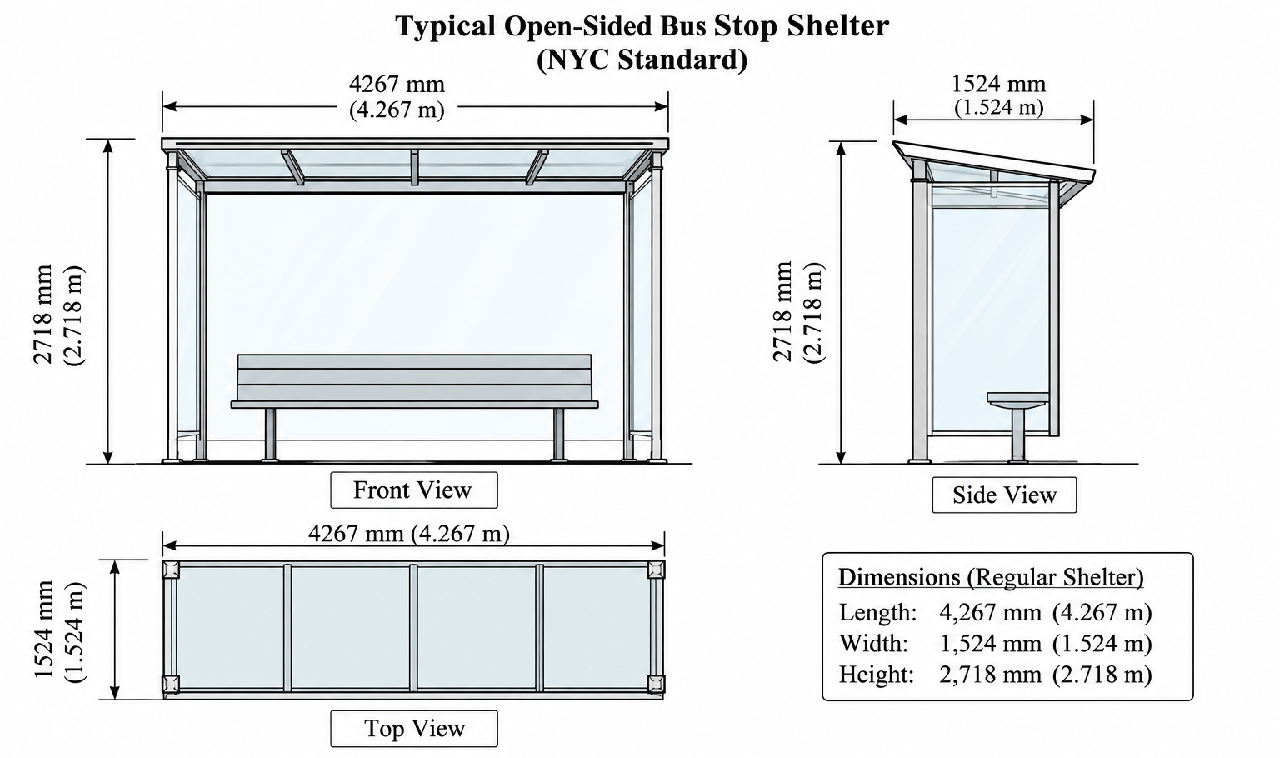
\includegraphics[width=\linewidth]{figures/07_bus_shelter_geometry.pdf}
\caption{Adopted NYC shelter dimensions \cite{nycshelter}.}
\label{fig:shelter-geometry}
\end{minipage}\hfill
\begin{minipage}[t]{0.49\linewidth}
\centering
\includegraphics[width=\linewidth]{figures/08_shelter_zoning.pdf}
\caption{Equal near/middle/edge accounting strips.}
\label{fig:shelter-zones}
\end{minipage}
\end{figure}

The problem's $3\,^{\circ}\mathrm C$ fan effect describes perceived cooling; B/C's $5/8\,^{\circ}\mathrm C$ describe air cooling \cite{problem}. We interpret the listed kW/hr numbers as powers $p_{A/B/C}=0.25/1.2/2.5$ kW. Tables~\ref{tab:bus-assumptions}--\ref{tab:bus-fields} specify the comparison: $34\,^{\circ}\mathrm C$, RH $30/70\%$, $T_r=36\,^{\circ}\mathrm C$ and 12 mean occupants. Geometry enters once through $n_z=\rho_zA_z$ when density replaces headcount.

\subsection{From device outlet to occupied air}
A changes prescribed local speed while retaining background temperature and moisture in the zero-local-heat base case \cite{fanguide}. For B/C, wet-bulb temperature bounds evaporation \cite{evapequip}:
\begin{equation}
 T_{o,s}=T_b-\min\{\Delta T_s^{\max},\;\varepsilon_s(T_b-T_{wb,b})\},
 \qquad s\in\{B,C\},
\label{eq:outlet}
\end{equation}
$b$ denotes the inlet background; $\varepsilon_s$ is evaporative effectiveness and $\Delta T_{B/C}^{\max}=5/8\,^{\circ}\mathrm C$ are the adopted outlet caps. With $\phi$ as RH fraction and pressures in Pa, SI psychrometrics give \cite{psychrolib}
\begin{align}
 w&=0.621945\frac{p_v}{p-p_v},\qquad p_v=\phi p_{sat}(T),\\
 h(T,w)&=1006T+w(2501000+1860T),
\label{eq:enthalpy}
\end{align}
Temperatures are in $^{\circ}$C. The near-isenthalpic evaporative stage, $h_{o,s}\simeq h_b$, yields
\begin{equation}
 w_{o,s}=\frac{h_b-1006T_{o,s}}{2501000+1860T_{o,s}}.
\end{equation}
This stage precedes electrical heating and neglects make-up-water enthalpy \cite{evap}. A device supply mixes with entrained background in a negligible-storage local region. For $x\in\{h,w\}$,
\begin{equation}
 0=\dot m_{s,z}(x_s^{\rm sup}-x_{\ell,s,z})+
 \dot m_{e,z}(x_b-x_{\ell,s,z}),\qquad
 \beta_{s,z}=\frac{\dot m_{s,z}}{\dot m_{s,z}+\dot m_{e,z}}.
\label{eq:delivery-balance}
\end{equation}
$\beta$ is a dry-air flow fraction, not a fraction of passengers or total flow assigned to a strip. A fraction $\chi$ of unit electric power $P_s=1000p_s$ W heats unit supply flow $\dot m_s$ before reaching people:
\begin{equation}
 h_s^{\rm sup}=h_{o,s}+\chi P_s/\dot m_s,\qquad
 w_s^{\rm sup}=w_{o,s},\qquad 0\leq\chi\leq1.
\label{eq:supply-heat}
\end{equation}
For A, the unheated outlet equals the inlet. Mixing conserves $h,w$, after which temperature and RH are recovered:
\begin{align}
 w_{\ell,s,z}&=(1-\beta_{s,z})w_b+\beta_{s,z}w_s^{\rm sup},\\
 h_{\ell,s,z}&=(1-\beta_{s,z})h_b+\beta_{s,z}h_s^{\rm sup},\\
 T_{\ell,s,z}&=\frac{h_{\ell,s,z}-2501000w_{\ell,s,z}}{1006+1860w_{\ell,s,z}}.
\label{eq:mixing}
\end{align}
RH is not averaged directly. The bus uses $b=a$ and $\chi=0$. Its B/C fractions imply entrainment-to-supply ratios $(1-\beta)/\beta=0.25/1.22/9.00$ and $0.11/0.43/1.50$. Parallel strip branches share one device's total supply.

\subsection{A common response and efficiency measure}
Standard effective temperature (SET) combines air temperature, radiation, airspeed and humidity for the reference passenger \cite{thermalcomfort,pythermal}:
\begin{equation}
 \Theta_{s,z}=F_{\mathrm{SET}}(T_{\ell,s,z},T_{r,z},v_{s,z},\phi_{\ell,s,z};\mathrm{met},\mathrm{clo}).
\label{eq:set}
\end{equation}
For the assumed hot-discomfort reference $\Theta_c=26\,^{\circ}\mathrm C$, define
\begin{equation}
 D(\Theta)=[\Theta-\Theta_c]_+,\qquad [x]_+=\max(x,0).
\end{equation}
Against the same shelter without active cooling, the signed improvement is
\begin{equation}
 b_{s,z,k}=D(\Theta_{0,z,k})-D(\Theta_{s,z,k}).
\end{equation}
Adverse effects remain negative. With $n_{z,k}$ people and time steps $\Delta t_k$ in hours,
\begin{align}
 U_s&=\sum_k\sum_z n_{z,k}b_{s,z,k}\Delta t_k, &
 E_s&=\sum_k p_{s,k}\Delta t_k,\\
 \eta_s&=U_s/E_s,\qquad E_s>0.
\label{eq:bus-efficiency}
\end{align}
Here $E$ is kWh and $\eta$ is person$\cdot{}^{\circ}\mathrm C\cdot$h/kWh, not COP. Empty zones earn no service; the zero-energy baseline has no ratio. The residual provides an accounting check:
\begin{equation}
 R_s=\sum_k\sum_z n_{z,k}D(\Theta_{s,z,k})\Delta t_k,
 \qquad \overline R_s=\frac{R_s}{\sum_k\sum_z n_{z,k}\Delta t_k}.
\label{eq:remaining}
\end{equation}
Thus $U_s+R_s=R_0$. We rank efficiency by $\eta$; overall adequacy enters Section~\ref{sec:effectiveness}. Under common operating time, the power ratios give delivery-independent break-even conditions:
\begin{equation}
\begin{aligned}
 \eta_B>\eta_A&\iff U_B>4.8U_A,\\
 \eta_C>\eta_A&\iff U_C>10U_A,\\
 \eta_C>\eta_B&\iff U_C>\frac{25}{12}U_B.
\end{aligned}
\label{eq:break-even}
\end{equation}

\subsection{Results: humidity and spatial delivery}
\begin{figure}[!ht]
\centering
\includegraphics[width=0.88\linewidth]{figures/01_local_conditions.pdf}
\caption{Local conditions under the bus inputs: A changes SET through airflow; B/C also change temperature and moisture.}
\label{fig:bus-local}
\end{figure}
For C, dry-case SET rises from $26.3\,^{\circ}\mathrm C$ near the outlet to $29.4\,^{\circ}\mathrm C$ at the edge; at RH $70\%$, it rises from $33.1$ to $35.2\,^{\circ}\mathrm C$. These gradients explain why a single air-temperature drop misses delivered service.

\begin{figure}[!ht]
\centering
\includegraphics[width=0.76\linewidth]{figures/24_bus_efficiency.pdf}
\caption{Uniform-occupancy efficiency: A leads both nominal humidity cases.}
\label{fig:bus-efficiency}
\end{figure}
Dry-case efficiencies are $84.6/24.5/21.1$ for A/B/C; humid-case values are $90.6/21.1/15.2$ (Figure~\ref{fig:bus-efficiency}). B/C outlet drops fall from $5/8\,^{\circ}\mathrm C$ to about $3.4/3.4\,^{\circ}\mathrm C$, as their common wet-bulb limit replaces the caps.

\begin{figure}[!ht]
\centering
\includegraphics[width=0.88\linewidth]{figures/03_humidity_sweep.pdf}
\caption{Humidity changes evaporative potential and SET-based efficiency at fixed delivery and demand.}
\label{fig:bus-humidity}
\end{figure}
Moving the same 12 people toward the edge lowers dry-case A efficiency from $118.3$ to $48.3$ and reverses B/C ordering: $24.5>21.1$ under uniform occupancy becomes $15.5<16.6$ under edge-heavy occupancy. A leads all six nominal climate--occupancy cases.

\subsection{Delivery failure and robustness}
Aiming or obstruction can weaken delivered airflow without reducing power. Holding $p_A=0.25$ kW, test
\begin{equation}
 v_{A,z}(q)=v_0+q(v_{A,z}^{\mathrm{nom}}-v_0),\qquad 0\leq q\leq1,
\end{equation}
$q$ is a delivery factor, not a motor-speed setting. On the sampled grid, A first wins at $q=0.18$ for RH $30\%$ and $0.16$ for RH $70\%$; the threshold lies within the preceding $0.02$ interval. B wins below it.

\begin{figure}[!ht]
\centering
\includegraphics[width=0.79\linewidth]{figures/05_delivery_decision.pdf}
\caption{Efficiency winner for RH $20$--$80\%$ and delivered-speed factor $q$; C wins no cell of this grid.}
\label{fig:bus-decision}
\end{figure}
One-factor endpoint tests give maximum B/A and C/A efficiency ratios $0.432$ and $0.372$. Including full local electric heating ($\chi=1$) changes dry-case efficiencies to $81.0/20.8/18.0$ and humid values to $86.8/17.4/12.1$; A remains first under those inputs. Psychrometric round trips, mass/enthalpy closure, $U+R=R_0$, zero-occupancy and signed-adverse checks pass. The delivery-loss reversal identifies a stronger sensitivity than these individual endpoint perturbations.
\subsection{Extreme dry heat: testing the efficiency ranking}
We test $T_a=T_r=40\,^{\circ}\mathrm C$ at RH 15\% and 20\%, retaining the device powers, delivery profiles, 5/8$\,^{\circ}\mathrm C$ outlet caps, and uniform occupancy. Figure~\ref{fig:extreme-heat} shows $\eta_A>\eta_B>\eta_C$ in both cases. At RH 15\%, the mean SET reductions are 1.43, 1.95, and 3.42$\,^{\circ}\mathrm C$, whereas the efficiencies are 68.43, 19.48, and 16.41 person$\cdot{}^{\circ}\mathrm C\cdot$h/kWh. C produces greater relief per passenger, but consumes ten times A's electricity. SET relief explains the service numerator; $\eta$ remains the comparison criterion.

The heat balance explains why dry-bulb cooling alone cannot establish the ranking. When air is warmer than the exposed skin or clothing surface, faster flow increases convective heat gain; it also promotes evaporative heat loss. SET combines these competing exchanges rather than imposing a temperature-triggered reversal of fan performance \cite{thermalcomfort}.

\begin{figure}[htbp]
\centering
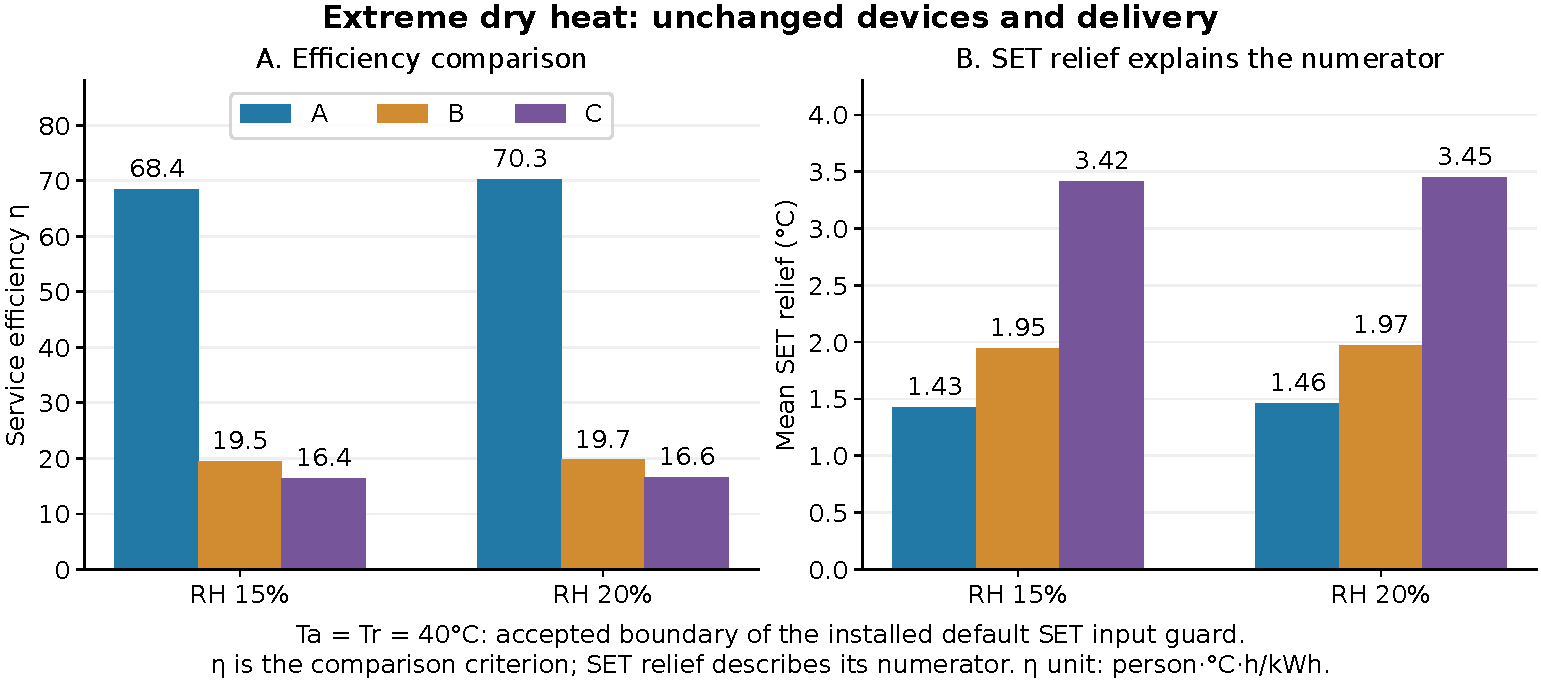
\includegraphics[width=.85\textwidth]{figures/26_extreme_heat.pdf}
\caption{Extreme dry-heat boundary test with the original device powers and delivery profiles. The left panel compares cooling efficiency; the right panel explains its SET-relief numerator. Inputs follow Assumption A4.}
\label{fig:extreme-heat}
\end{figure}


\section[Rail station]{Canberra Station: Dynamic Background and Local Service}
\label{sec:rail}

\subsection{From a fixed reservoir to coupled zones}
Canberra MRT is an elevated, naturally ventilated station in Singapore \cite{canberra-rsp,canberra-lta}. Using its approximate $L=220$ m length with assumed aggregate waiting width $b=6$ m and usable fraction $\alpha=0.8$ gives
\begin{equation}
 A_{\mathrm{occ}}=\alpha Lb=1056\,\mathrm{m^2}.
\label{eq:canberra-area}
\end{equation}
Three access/core/edge zones each have $352\,\mathrm{m^2}$ and, at 4 m effective height, $1408\,\mathrm{m^3}$. Table~\ref{tab:rail-inputs} defines the $33\,^{\circ}\mathrm C$, RH $70\%$ comparison. Its $4$--$10$ h$^{-1}$ background exchange implies 6--15 min replacement times, comparable to the 15-min passenger cycle: storage and humidity feedback must now be resolved.

\begin{figure}[!ht]
\centering
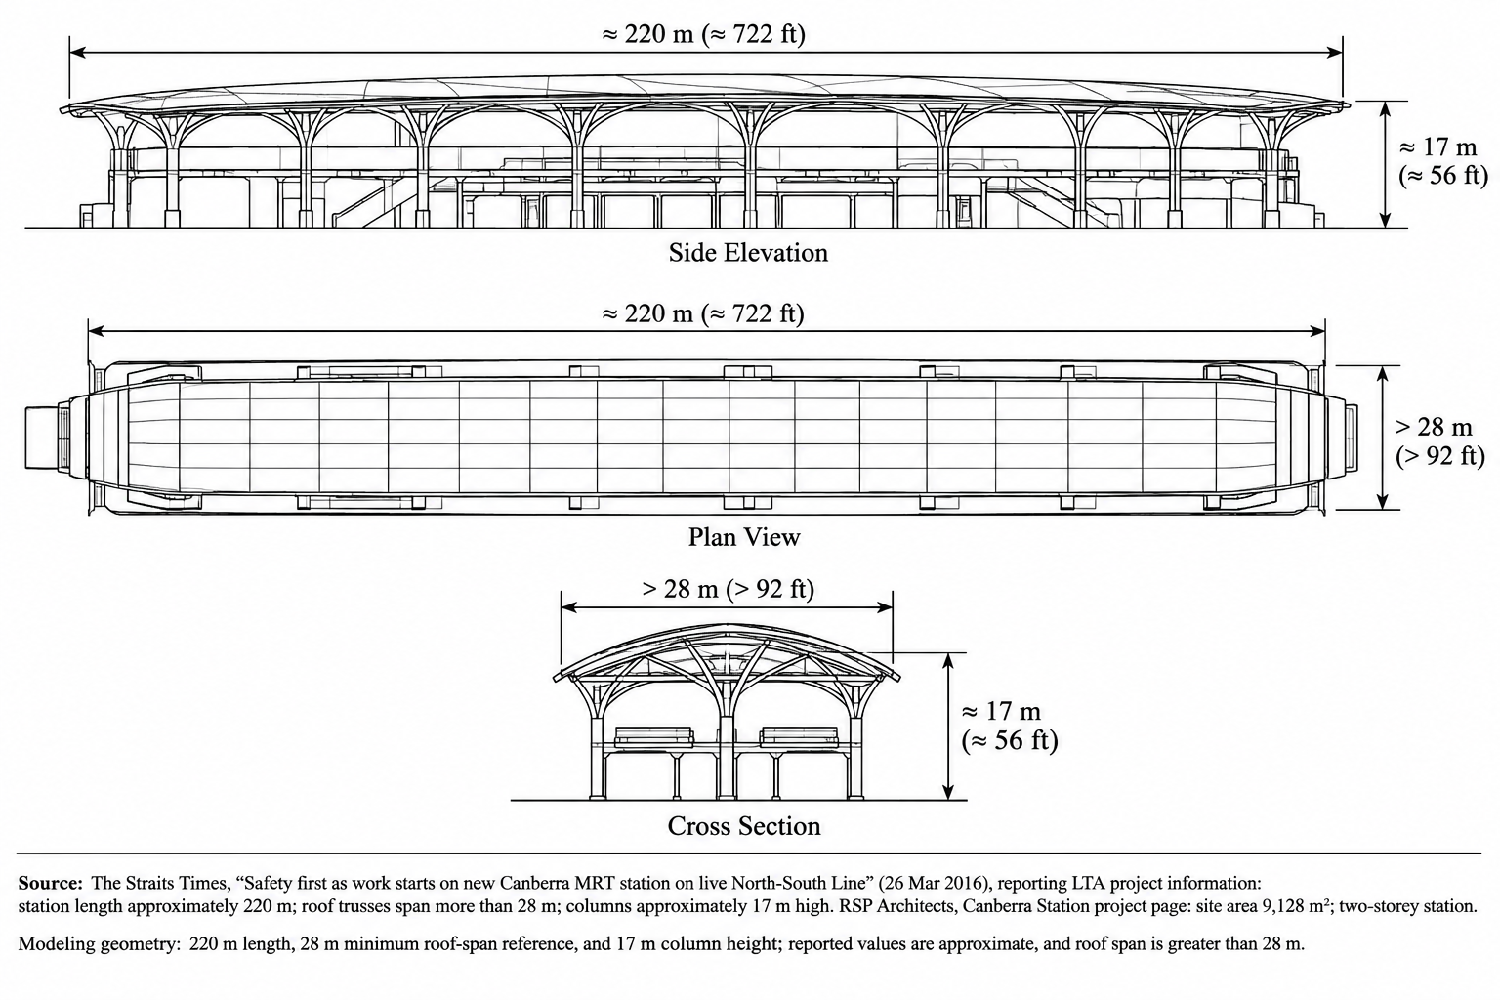
\includegraphics[width=0.66\linewidth]{figures/13_canberra_station.pdf}
\caption{Canberra station context. Structural dimensions guide scale; the three waiting zones are modeled separately \cite{canberra-dimensions,canberra-rsp}.}
\label{fig:canberra}
\end{figure}

Each zone retains $h_z,w_z$ and effective surface temperature $T_{m,z}$, with constant reference dry-air mass $M_z=\rho_{da,o}V_z$. The device, local-mixing and SET operators remain those of the bus. For $x=h$ or $w$, balanced exchange is
\begin{equation}
 \mathcal L_z(x)=\dot m_{0z}(x_o-x_z)+\sum_{j\ne z}\dot m_{zj}(x_j-x_z),
 \qquad \dot m_{0z}=M_z\lambda_z/3600.
\label{eq:rail-exchange}
\end{equation}
$\lambda_z$ is ACH in h$^{-1}$; interzone rates satisfy $\dot m_{zj}=\dot m_{jz}$. Outdoor exchange represents wind/opening effects through the prescribed cycle \cite{ventilation}. With time in seconds, the three conservation equations per zone are \cite{epzone}
\begin{align}
 M_z\dot h_z={}&\mathcal L_z(h)+H_{ma,z}(T_{m,z}-T_z)
 +n_zq_c+n_zg h_v(T_z)+P_z
 +\sum_k x_{zk}\dot m_k(h_{e,zk}-h_z),\label{eq:rail-enthalpy}\\
 M_z\dot w_z={}&\mathcal L_z(w)+n_zg+
 \sum_k x_{zk}\dot m_k(w_{e,zk}-w_z),\label{eq:rail-moisture}\\
 C_{m,z}\dot T_{m,z}={}&H_{mo,z}(T_o-T_{m,z})+Q_{\mathrm{sol},z}
 +n_zq_r-H_{ma,z}(T_{m,z}-T_z).\label{eq:rail-surface}
\end{align}
Here $n_z$ is occupancy; per-person $q_c,q_r$ are convective/radiant W and $g$ is vapor kg/s. Vapor enthalpy is $h_v(T)=2501000+1860T$ J/kg, with no second latent term. $H_{ma},H_{mo}$ are W/K, $C_m$ is J/K, $Q_{\rm sol}$ is W, and $P_z=\sum_kx_{zk}P_k$ with $P_k=1000p_k$ W. Subscript $e$ denotes the unheated device outlet (the bus's $o,s$), so A has no evaporative source; B/C add moisture while approximately conserving outlet enthalpy. Surface exchange cancels between the air and wall budgets.

Recover $T_z=(h_z-2501000w_z)/(1006+1860w_z)$; effective view fraction $F_z$ determines mean radiant temperature \cite{thermalcomfort}:
\begin{equation}
 T_{r,z}=\left[F_z(T_{m,z}+273.15)^4+(1-F_z)(T_{r,o}+273.15)^4\right]^{1/4}-273.15.
\label{eq:rail-mrt}
\end{equation}
The separate outdoor radiant input is $T_{r,o}$. Increasing $w_z$ reduces the next device pass's wet-bulb depression, providing the feedback absent from the fixed-background bus.

\subsection{Local delivery with exact return accounting}
Device flow and entrained background return to their original zone. For finite entrainment ($\beta>0$), the local mixing equations imply
\begin{align}
 (\dot m_k+\dot m_e)(h_{\ell,zk}-h_z)+(1-\chi)P_k
 &=\dot m_k(h_{e,zk}-h_z)+P_k,\\
 (\dot m_k+\dot m_e)(w_{\ell,zk}-w_z)
 &=\dot m_k(w_{e,zk}-w_z).
\label{eq:return-closure}
\end{align}
Thus the local exposure calculation preserves the existing net heat and moisture sources exactly. Covered people use local $T,\phi,v$; uncovered people use background $T,\phi,v_0$, and both share $T_r$. Here $\beta=0.5$, $\chi=1$ and A/B/C unit flows are $0.6/0.6/1.2$ kg dry air/s under Table~\ref{tab:rail-inputs}; $\chi=1$ places all electrical heat in supply before passengers.

Two reductions identify the inheritance precisely. At $\beta=0$, the scalar exposure becomes the original shared-background calculation while prescribed speeds remain. Fixing background to outdoor $h_a,w_a$, using bus radiation, speeds, occupancy and $\beta$, and setting $\chi=0$ recovers the bus calculation exactly. Setting time derivatives to zero alone would not impose that reservoir boundary.

\subsection{Counts, coverage and efficiency}
Let $s$ index an installation and $x_{zk}$ its nonnegative integer count of type $k$ in zone $z$. For unit footprints $a_{A/B/C}=20/30/40\,\mathrm{m^2}$, uniform zone density gives
\begin{equation}
 c_{zk}=\frac{x_{zk}a_k}{A_z},\qquad
 c_{z0}=1-\sum_k c_{zk}\ge0,\qquad \sum_kx_{zk}a_k\le A_z.
\label{eq:coverage}
\end{equation}
These passenger fractions $c$ differ from the air-mixing fraction $\beta$. Average discomfort across subgroups, not velocities or device efficiencies:
\begin{equation}
 \overline D_{s,z}(t)=c_{z0}D[\Theta(T_z,T_{r,z},v_0,\phi_z)]
 +\sum_k c_{zk}D[\Theta(T_{\ell,zk},T_{r,z},v_{zk},\phi_{\ell,zk})].
\label{eq:mixed-discomfort}
\end{equation}
All units affect the background; direct coverage determines the additional local exposure. Every plan starts after the same two-hour uncooled warm-up, runs two hours, and uses a matched no-device baseline. The common passenger history totals 440 person-hours. With $p_k$ in kW,
\begin{align}
 U_s&=\frac1{3600}\int_0^{7200}\sum_z n_z(t)[D_{0,z}(t)-\overline D_{s,z}(t)]\,dt,\\
 E_s&=\frac1{3600}\int_0^{7200}\sum_{z,k}x_{zk}p_k\,dt,
 \qquad \eta_s=U_s/E_s.
\label{eq:rail-efficiency}
\end{align}
The $1/3600$ factors convert seconds to hours, retaining person$\cdot{}^{\circ}\mathrm C\cdot$h/kWh. This section compares $U/E$. Mean residual $\overline R_s=\int\sum_z n_z\overline D_{s,z}\,dt/\int\sum_z n_z\,dt$ supplies the later adequacy criterion in Section~\ref{sec:effectiveness}.

\subsection{Deployment results and verification}
\input{sections/unified_results}

\begin{figure}[!ht]
\centering
\includegraphics[width=0.88\linewidth]{figures/22_station_efficiency.pdf}
\caption{A3 leads all 24 sampled installations; A36 leads the six equal-coverage benchmarks. Device counts change both delivered service and background loads.}
\label{fig:deployment-efficiency}
\end{figure}

\begin{figure}[!ht]
\centering
\includegraphics[width=0.88\linewidth]{figures/23_delivery_efficiency.pdf}
\caption{Efficiency sensitivity to mixing and heat allocation; background trajectories remain unchanged by the local mapping.}
\label{fig:local-sensitivity}
\end{figure}

Global energy/moisture budgets and local return identities close numerically. Halving the time step changes the tested mixed-plan efficiencies by at most $5.4\times10^{-6}$ relatively; $\beta=0$ reproduces all 24 former shared-background results exactly. The fixed-reservoir test recovers bus states and service. These checks verify the extension's conservation and reduction properties.
\FloatBarrier
\IfFileExists{sections/applications.tex}{\section[Venue applications and scale]{Apply the Model: From a Ticket Queue to Fremont Street}
\label{sec:applications}
\input{sections/task3_values}

\subsection{Two service areas, a 140-fold difference in size}
\textbf{Fremont Street Experience, Las Vegas}, provides a large covered pedestrian setting: its official canopy length is 1,375 ft, or 419.1 m \cite{fremont-canopy}. Our three demand zones span an $8382$-m$^2$ occupied strip. At the \textbf{Honolulu Zoo entrance}, the architect explicitly designed shaded ticket-purchasing and queuing space \cite{honolulu-zoo-entrance}; the modeled service boundary is the $60$-m$^2$ public queue outside the ticket window. The area ratio is $139.7$. Las Vegas supplies the dry-desert case; Honolulu supplies a warm coastal case with a separate natural-wind sensitivity \cite{las-vegas-climate,honolulu-climate}. Geometry, attendance and weather inputs are collected in Table~\ref{tab:venue-inputs}.

\begin{figure}[!ht]
\centering\includegraphics[width=.94\linewidth]{figures/31_venue_layouts.pdf}
\caption{Analytical service boundaries and prescribed attendance. Fremont has three demand zones; the ticket queue has one. The three local delivery strips belong to each device footprint, independently of this site partition.}
\label{fig:venue-layouts}
\end{figure}

\subsection{Transfer the physical kernel, then aggregate service}
We use the fixed-reservoir limit of the station model: outdoor $h,w,T_r$ are prescribed, while its integer allocation and coverage calculation are retained. Each unit uses the same wet-bulb-limited outlet, conservative local mixing and SET response as in Task 2. The three strip responses are averaged \emph{after} conversion to excess SET. Let $\delta_k=\frac13\sum_{j=1}^3[D_0-D(\Theta_{kj})]$ be the mean relief inside a complete footprint, and $\mathcal H_z=\int_0^H n_z(t)\,dt$ the zone's visitor-hours. Then
\begin{equation}
 u_{zk}=\mathcal H_z\frac{a_k}{A_z}\delta_k,\qquad
 U_s=\sum_{z,k}x_{zk}u_{zk},\qquad E_s=H\sum_{z,k}x_{zk}p_k.
\label{eq:venue-service}
\end{equation}
Time is measured in hours, giving $3210$ and $96$ visitor-hours in Fremont and Honolulu. Person-time coverage is $q_s=\sum_z\mathcal H_z\sum_k c_{zk}/\sum_z\mathcal H_z$. All installed units run throughout the four-hour period; water supply is counted once per unit. The disjoint-footprint condition in Eq.~\eqref{eq:coverage} prevents double-counting people.

This linear service structure also solves the efficiency-only allocation problem. For every positive-energy layout,
\begin{equation}
 \eta_s=\sum_{z,k}\frac{Hx_{zk}p_k}{E_s}\,
                  \frac{u_{zk}}{Hp_k}
 \ \le\ \max_{z,k}\frac{u_{zk}}{Hp_k}.
\label{eq:venue-bound}
\end{equation}
The bound is attained by one unit of the maximizing type in the maximizing zone whenever its footprint fits. It yields \textbf{$\FMaxEta$ in Fremont and $\HMaxEta$ in Honolulu} person$\cdot{}^\circ$C$\cdot$h/kWh, attained by A in Fremont's middle demand zone and A in the ticket queue. Their coverages are $0.33\%$ and $33.33\%$. Additional A units within the same zone tie while their footprints fit. This efficiency result uses the entire integer domain, without a service-coverage or cost threshold.

\subsection{Climate changes the relative value of the devices}
Table~\ref{tab:venue-results} compares the largest pure-type installations that fit each site. Honolulu admits three A units, two B units or one C unit: the last serves only two-thirds of the queue. Every unit's full power remains in the denominator.
\input{sections/task3_results_table}

The wet-bulb temperatures are $\FTwb^\circ$C and $\HTwb^\circ$C. C's outlet drop reaches $\FCDrop^\circ$C in Fremont and $\HCDrop^\circ$C in Honolulu. At the dry site, C's larger temperature reduction and delivery profile outweigh its extra power relative to B; at the coastal site, B supplies more useful service per kWh than C. A retains the highest efficiency in both nominal cases. These rankings follow from local exposure and electricity together.

\begin{figure}[!ht]
\centering\includegraphics[width=.96\linewidth]{figures/27_venue_comparison.pdf}
\caption{Pure-type installations: useful service per kWh and mean SET-excess relief across all visitors. Coverage differences, including Honolulu C1's uncovered third, remain in the service calculation.}
\label{fig:venue-comparison}
\end{figure}

Honolulu's larger efficiency values also reflect its greater visitor density. To isolate the climate effect, we exchange $(T_a,\mathrm{RH},T_r,v_0)$ between sites while holding geometry, attendance and device counts fixed. The B--C order follows the weather tuple in both transfers. At Honolulu's density, A's efficiency changes from $\HMaxEta$ under its own weather to $\HWithFEta$ under Fremont's weather. Thus a high site-level $\eta$ cannot be attributed to favorable climate alone.

Natural wind also changes the marginal value of equipment: raising Fremont's background speed from $.20$ to $.80$ m/s changes the efficiency-maximizing type from A to C, with a new bound of $5.38$. The uncooled baseline SET falls from $33.77$ to $31.51^\circ$C. Extra fan speed brings less benefit when ambient air is already moving, whereas evaporative temperature reduction remains available.

\subsection{Controlled scaling and the finite-footprint limit}
For a fixed climate and unchanged local delivery, multiply each zone's area and visitor-hours by $\lambda$. With the original devices, each footprint contains the same number of people, so $U$ and $E$ remain constant while person-time coverage becomes $q/\lambda$. Replicating devices as well gives
\begin{equation}
 (A_z,\mathcal H_z,x_{zk})\mapsto
 (\lambda A_z,\lambda\mathcal H_z,\lambda x_{zk})
 \quad\Longrightarrow\quad
 (U,E,q,\eta)\mapsto(\lambda U,\lambda E,q,\eta).
\label{eq:venue-scale}
\end{equation}
Integer multipliers preserve feasible counts. For the Honolulu A3 reference, scaling from 60 to 480 m$^2$ with attendance at the same density leaves $\eta=\HMaxEta$. Three fixed fans reduce coverage from $100\%$ to $12.5\%$; 24 fans restore full coverage and raise four-hour electricity from 3 to 24 kWh. These are controlled similarity properties of the model, separating scale from climate.

\begin{figure}[!ht]
\centering\includegraphics[width=.96\linewidth]{figures/30_scale_transfer.pdf}
\caption{Controlled scale and boundary tests. Proportional deployment preserves efficiency and coverage; fixed equipment preserves efficiency but loses coverage. In the separate single-unit test, reducing available area clips the far delivery strip first, with the full unit power still charged.}
\label{fig:venue-scaling}
\end{figure}

Small spaces also expose a finite-footprint limit. We retain only the portions of the near, middle and far strips lying within the service boundary and recompute their area-weighted relief. The efficiency plateaus once a complete footprint fits; below that size, lost served area changes the result even at unchanged visitor density. Therefore the transferable characteristics are \textbf{occupied density, retained local delivery, wet-bulb depression and footprint fit}. Geometry sets who benefits; climate sets the benefit per exposed person. Matched-baseline identities, valid local air states and the scaling relations are checked against the exported calculations.
\FloatBarrier
}{}
\IfFileExists{sections/effectiveness_complete.tex}{\input{sections/effectiveness_complete}}{}
\IfFileExists{sections/operator_memo.tex}{\input{sections/operator_memo}}{}
\IfFileExists{sections/public_blog.tex}{\clearpage
\section*{Public Blog: How Much Comfort Does One Kilowatt-Hour Buy?}
\addcontentsline{toc}{section}{Public blog}

An outdoor fan can help people feel cooler while the air thermometer barely changes. An evaporative cooler lowers air temperature while adding moisture. A fair comparison follows the cooling to the visitor: what temperature, humidity, air movement and radiant heat reach that person, and for how long?

Our model combines those influences using Standard Effective Temperature, or SET. One service unit means reducing one person's SET excess by one degree for one hour. Dividing that benefit by electricity gives cooling efficiency. It measures relief accumulated over visitor-hours.

We applied the same calculation to two very different spaces: a large occupied corridor under the Fremont Street Experience canopy in Las Vegas, and a shaded ticket queue at Honolulu Zoo \cite{fremont-canopy,honolulu-zoo-entrance}. The modeled areas are 8382 and 60 square meters. Las Vegas offers dry heat; Honolulu offers a warm, humid coastal setting. The smaller queue also packs more visitor-time into each square meter, which helps each unit serve more people.

At Honolulu, three fans cover the queue and deliver about \textbf{143 service units using 3 kWh}: roughly \textbf{48 units per kWh}. In Fremont, placing one fan in the busiest demand zone yields about \textbf{17 units per kWh}, but directly serves only \textbf{0.33\% of visitor-time} across the corridor. A good efficiency ratio can coexist with very limited coverage. More equipment in the same busy zone can retain that ratio while serving more people.

Choosing a practical installation adds another question: how much service must it provide, and at what cost? Our illustrative policy requires at least 80\% coverage and $1.5^\circ$C average relief, alongside space and electricity limits. It selects 266 fans plus 16 evaporative units in Fremont, and one fan plus one evaporative unit in Honolulu. In the queue, three fans already deliver $1.4908^\circ$C relief. Lowering the target from $1.50$ to $1.49^\circ$C changes the least-cost answer to fans alone.

Scale brings a similar distinction. If Honolulu's area and crowd both grow eightfold, keeping three fans preserves their efficiency but lowers coverage from 100\% to 12.5\%. Twenty-four fans restore coverage. The useful questions are therefore connected: how much benefit does each kWh buy, who receives it, and what service can the operator afford? During severe heat, also follow local advisories and adjust outdoor plans \cite{nws-heat}.
}{}
\clearpage
\phantomsection\addcontentsline{toc}{section}{References}
\begin{thebibliography}{99}
\fontsize{9.5}{11}\selectfont
\urlstyle{same}
\setlength{\itemsep}{0pt}
\setlength{\parskip}{0pt}
\bibitem{ashrae}
ASHRAE. \emph{2026 ASHRAE Handbook---Refrigeration},
Chapter 15, \emph{Retail Food Store Refrigeration and Equipment}.
Product Temperatures and Display Refrigerator Cooling Load sections.
\url{https://handbook.ashrae.org/Handbooks/R26/IP/r26_ch15/r26_ch15_ip.aspx}.


\bibitem{etl}
UK Department for Energy Security and Net Zero.
\emph{Energy Technology List: Retrofit Measures for Open Fronted Refrigerated Display Cabinets}.
Definitions and product-temperature performance requirements.
\url{https://etl.energysecurity.gov.uk/products/refrigeration-equipment/retrofit-measures-open-fronted-refrigerated-display-cabinets}.


\bibitem{evap}
ASHRAE. \emph{2023 ASHRAE Handbook---HVAC Applications},
Chapter 53, \emph{Evaporative Cooling}.
\url{https://handbook.ashrae.org/Handbooks/A23/SI/A23_Ch53/a23_ch53_si.aspx}.


\bibitem{problem}
COMAP. \emph{2026 HiMCM Problem B: Air Conditioning the Environment: Modeling Energy Waste in Public Cooling}.
Requirements 1--5.

\bibitem{evapequip}
ASHRAE. \emph{2020 ASHRAE Handbook---HVAC Systems and Equipment},
Chapter 41, \emph{Evaporative Air-Cooling Equipment}, Section 1.
\url{https://handbook.ashrae.org/handbooks/S20/SI/s20_ch41/s20_ch41_si.aspx}.


\bibitem{fanguide}
Center for the Built Environment, University of California, Berkeley.
\emph{Fans for Cooling People Guidebook: Elevated Air Speed and Thermal Comfort}.
\url{https://cbe-berkeley.gitbook.io/fans-guidebook/full-guidebook/elevated-air-speed-and-thermal-comfort}.


\bibitem{thermalcomfort}
ASHRAE. \emph{2017 ASHRAE Handbook---Fundamentals},
Chapter 9, \emph{Thermal Comfort}, Section 10, Environmental Indices.
\url{https://handbook.ashrae.org/Handbooks/f17/IP/f17_ch09/f17_ch09_ip.aspx}.


\bibitem{pythermal}
Tartarini, F., and Schiavon, S. (2020).
pythermalcomfort: A Python package for thermal comfort research.
\emph{SoftwareX}, 12, 100578.
\url{https://doi.org/10.1016/j.softx.2020.100578}.
SET API and applicability limits:
\url{https://pythermalcomfort.readthedocs.io/en/stable/documentation/models.html}.


\bibitem{psychrolib}
Meyer, D., and Thevenard, D. (2019).
PsychroLib: a library of psychrometric functions to calculate thermodynamic properties of air.
\emph{Journal of Open Source Software}, 4(33), 1137.
\url{https://doi.org/10.21105/joss.01137}.
SI psychrometric API:
\url{https://psychrometrics.github.io/psychrolib/api_docs.html}.


\bibitem{nycshelter}
New York City Department of Transportation.
\emph{Street Design Manual: Bus Stop Shelter}, Description (regular-size shelter).
\url{https://www.nycstreetdesign.info/furniture/bus-stop-shelter}.


\bibitem{hillphoenix}
Hillphoenix. \emph{CF-R/CF-FS-R/CF-S-R Multi-Deck Merchandiser: Installation \& Operations Manual}, April 2021, Technical Reference, printed p.~4 (PDF p.~8).
\url{https://www.hillphoenix.com/wp-content/uploads/2021/06/CF-S-R-display-case-manual.pdf}.
Product classification: \url{https://www.hillphoenix.com/products/cf}.


\bibitem{epzone}
EnergyPlus Development Team. \emph{Engineering Reference},
``Basis for the Zone and Air System Integration'' and ``Moisture Predictor-Corrector.''
\href{https://energyplus.readthedocs.io/en/latest/guides/engineering-reference/2.1-basis-for-the-zone-and-air-system-integration.html}{Online source};
\href{https://energyplus.readthedocs.io/en/latest/guides/engineering-reference/2.4-moisture-predictor-corrector.html}{Online source}.


\bibitem{cruz2026}
Cruz-Salas, M.V., Puerto, E., Rojas, J., Barrios, G., Huelsz, G., and Ram\'irez, G. (2026).
Mist evaporative cooling system with natural ventilation in a semi-outdoor environment: Theoretical models, experiments, and thermal simulations.
\emph{Energy and Buildings}, 366, 117700.
\url{https://doi.org/10.1016/j.enbuild.2026.117700}.

\bibitem{ventilation}
ASHRAE. \emph{2025 ASHRAE Handbook---Fundamentals}, Chapter 16,
\emph{Ventilation and Infiltration}, Section 10, Natural Ventilation.
\href{https://handbook.ashrae.org/Handbooks/F25/SI/F25_Ch16/F25_Ch16_si.aspx}{Online source}.


\bibitem{canberra-rsp}
RSP. \emph{Canberra Station}. Project description and site area.
\href{https://rsp.design/project/canberrastation/}{Online source}. 

\bibitem{canberra-lta}
Land Transport Authority. \emph{Stations, stations on the tracks, which is the greenest of them all?}
Canberra station: natural ventilation, planting, glazing and louvers.
\href{https://www.lta.gov.sg/content/ltagov/en/who_we_are/statistics_and_publications/Connect/greenmrtstations.html}{Online source}.


\bibitem{canberra-dimensions}
\emph{The Straits Times}. \emph{Safety first as work starts on new Canberra MRT station on `live' North-South Line}, March 26, 2016.
Source identified in the user-supplied schematic for approximate structural dimensions.
\href{https://www.straitstimes.com/singapore/safety-first-as-work-starts-on-new-canberra-mrt-station-on-live-north-south-line}{Online source}.

\bibitem{singapore-climate}
Meteorological Service Singapore. \emph{Climate of Singapore}. Temperature and humidity climatology.
\href{https://www.weather.gov.sg/climate-climate-of-singapore}{Online source}. 

\input{sections/references_venues}
\ifinlineai
\bibitem{codex} OpenAI. \emph{Codex}, model development, code, research, drafting and figures, November 2026. See Report on Use of AI Tools.
\bibitem{gemini} Google. \emph{Gemini}, user-supplied analysis excerpt, November 2026. See Report on Use of AI Tools.
\fi
\end{thebibliography}
\clearpage
\phantomsection\addcontentsline{toc}{section}{Report on Use of AI Tools}
\section*{Report on Use of AI Tools}
OpenAI Codex was used during November 2026 to assist with translation, model formulation, Python implementation, source research, English drafting, LaTeX preparation and figure generation. The user also supplied a Google Gemini analysis as a PDF excerpt; its process-oriented explanation informed the early organization. Gemini was not used as a scientific source for the physical equations or numerical inputs.

\noindent\textbf{Development record.} The assistance covered freezer service accounting; psychrometric and SET calculations; the shared local-delivery operator; station heat, moisture and surface balances; candidate deployment comparisons; scope separation between efficiency and effectiveness; and the final CP-SET restructuring. The supplied drawings and earlier award papers were used for context and presentation, with their data provenance distinguished from scenario inputs.

\noindent\textbf{Latest revision.} The user selected Fremont Street Experience and the Honolulu Zoo ticketing queue for a large--small venue comparison. Codex researched site identity and climate, specified the assumption table, implemented the shared CP-SET calculation, and generated climate-transfer, scale and boundary tests. The revision uses an analytical efficiency bound and integer cost optimization, with a separate enumeration audit for the small venue. Associated summaries, operating guidance and standalone PDF figures were updated from the computed results. The Python implementation, input files, CSV outputs, figure scripts and verification records are retained with the LaTeX project.

\noindent\textbf{Verification record.} Automated checks cover heat and water conservation, service-energy identities, limiting-case recovery, time-step convergence and consistency between tables, figures and outputs. The AI-assisted workflow performed these checks; independent team review is recorded separately by the team.

\noindent\textbf{Tool identification and transcript archive.} OpenAI Codex, accessed November 8, 2026; the session identifies Codex as based on GPT-6; a more specific deployment identifier was not supplied. Google Gemini, user-supplied conversation excerpt; the model identifier is not present in that excerpt. The original prompts and complete retained outputs are held in the associated conversation records. This narrative is an activity record, not a replacement for those transcripts.

\noindent\textbf{Policy reference.} COMAP, \emph{Use of AI Tools in COMAP Contests}, v102025, \url{https://www.contest.comap.com/undergraduate/contests/mcm/flyer/Contest_AI_Policy.pdf}; and 2026 HiMCM instructions, \url{https://www.contest.comap.org/highschool/contests/himcm/instructions.html}, accessed November 8, 2026.

\end{document}
